\documentclass{article}

\usepackage[utf8]{inputenc}
\usepackage[spanish]{babel}
\usepackage{graphicx}
\usepackage{amsmath}

\title{Modelos matemáticos discretos}
\author{Nelly Mariela Moreno Cruz}
\begin{document}
\maketitle
\section{Ecuaciones en diferencias}
\subsection{Primer orden}
Sabemos que: $$\lim_{x\to\infty}\frac{1}{x}=0$$

Calcular los valores propios de $$A=
\begin{pmatrix}
1 & 2\\
\pi & 4
\end{pmatrix}
$$



Ejemplo 1:
Consideremos el valor de una inversión de \$1000 que acumula interés de 1\% cada mes.
El valor de la inversión cuando han transcurrido $n$ meses es: $$x_n=(1000)(1.01)^n$$.
Una gráfica del resultado es:

\begin{center}
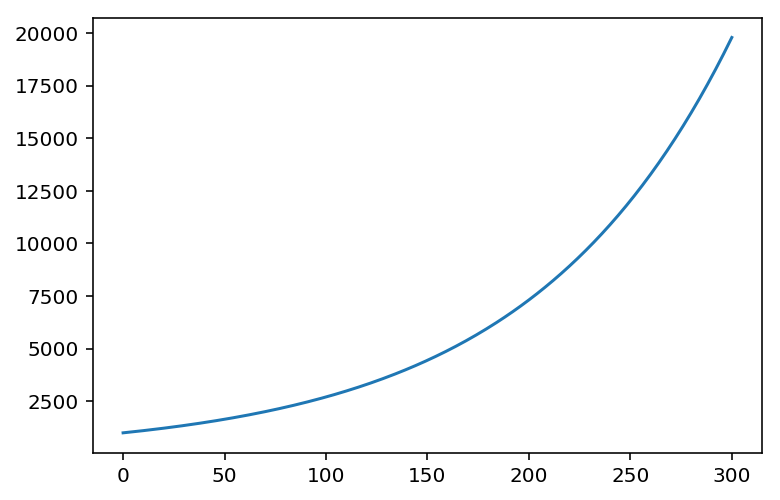
\includegraphics[width=10cm]{graficaa}
\end{center}

Para encontrar este resultado, ocupamos que:
$$\sum_{i=0}^{n-1}a^i=\frac{1-a^{n}}{1-a}$$.

Algunos valores de la inversión:

\begin{center}
\begin{tabular}{|c|l|}
\hline
Mes & Valor\\
\hline
0 & 1000\\
\hline
1 & 1010\\
\hline
2 & 1020.1\\
\hline
3 & 1030.301\\
\hline
4 & 1040.60401\\
\hline
\end{tabular}
\end{center}

\begin{center}
\huge
\textbf{Modelos}
\end{center}

\subsection{Segundo orden}
\end{document}

